\section{Grafana}

\begin{figure}[ht]
    \centering
    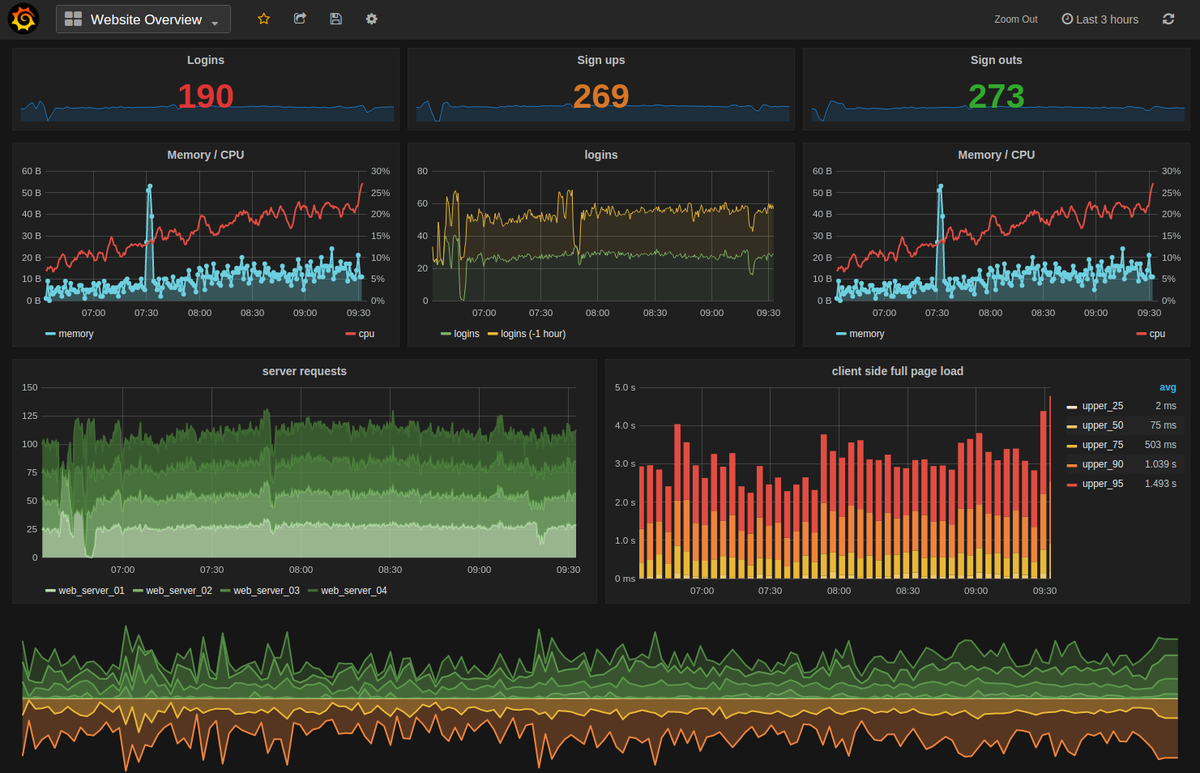
\includegraphics[width=\linewidth]{content/chapter_3/images/grafana_dashboard.png}
    \caption{Grafana Graph Visualization (Source: Flickr~\cite{file:screenshots_grafana})}
    \label{fig:grafana_dashboard}
\end{figure}
Grafana is a web-based analytics and interactive visualization application that runs on a variety of platforms. When connected to supported data sources, it produces web-based charts, graphs, and alerts. Grafana Enterprise, a paid version with more features, is available as a self-hosted installation or as a Grafana Labs cloud service account~\cite{Misc:grafana_labs_website}.
Grafana is split into two parts: a front end and a back end, both of which are built in TypeScript and Go and, through a plug-in, system, it can be expanded, adding specific customizations to the existing platform~\cite{Misc:grafana_docs}.
Using interactive query builders, end users can develop complicated monitoring dashboards. But what is a dashboard anyway?

\subsection{Dashboard what is it?}
A dashboard, in business, is a type of graphical user interface that often enables quick access to key performance indicators (KPIs) related to a certain goal or business activity.
In our context, ''dashboard'' refers to a ''progress report'' or ''report'' and, as a type of data visualization, it is mostly accessible by a web browser and is usually linked to regularly updating data sources.
The term dashboard is derived from the automotive dashboard, where drivers may monitor the primary functions at a glance using the instrument panel.

The success of dashboard projects depends on the relevancy/importance of information provided within the dashboard. This includes the metrics chosen to monitor and the timeliness of the data forming those metrics; data must be up-to-date and accurate.
Well known dashboards include Google Analytics dashboards, used on 55\% of all websites~\cite{Misch:w3techs_usage}, which show user activity on a website, or the UK government, and similar for each country, coronavirus tracker, for the COVID-19 pandemic~\cite{Misc:uk_covid_dash}.

An interesting project is the GLAM Wiki dashboard, from Israel~\cite{Misc:wikidata_glam_project}.
Its purpose is to assist GLAM institutions (galleries, libraries, archives, and museums) in tracking the use of their free-content files that they have submitted to Wikimedia projects.
Based on multiple specified indices and several time frames, the dashboard visualizes statistical data that shows the extent of exposure and usage of these public-domain assets.
The collecting data, which is presented in a variety of diagrams and graphs, allows the institutions to obtain insights, discover patterns and preferences, and understand the overall impact of these free materials on the global audience of Wikimedia-project users.

\subsection{Key strengths}
Now that we are familiar with the ''dashboard'' concept, we can highlight why we should use Grafana; here are some of the key features~\cite{Article:comprehensive_study_grafana}:
\begin{itemize}
    \item \textbf{Visualize} fast and flexible visualization with a variety of options allows data to be displayed the way the user wants it;
    \item \textbf{Dynamic Dashboard} dynamic and reusable dashboards may be created using template variables.
    \item \textbf{Explore Metric} ad-hoc queries and dynamic drill-down permits for data discovery.
          View splits and side-by-side comparisons of different time ranges and data sources is easily achievable;
    \item \textbf{Explore Logs} fast switch from metrics to logs preserving label filters. Furthermore, searching the logs is rather quick and can be performed on live streams;
    \item \textbf{Alerting} most of the vital/operational metrics may be alerted visually and different types of notifications (SMS, mail, Slack) may be despatched with the aid of Grafana;
    \item \textbf{Mixed Data Source} the same chart can have different data source: these can be selected based on queries, with built-in support for most of the prominent data sources available in the market as well as custom ones;
    \item \textbf{Annotations} graphs may have events that can be annotated, two solutions are possible:
          use native annotation store, with the ability to add annotation events directly from the graph panel or via the HTTP API, or querying other data sources.
          Event metadata and tags can be seen when hovering over events.
\end{itemize}

\paragraph{Loading speed of Grafana dashboards}
% \texttt{And how to keep it fast}
\todo{Potenzialmente da rimuovere/espandere}
Loading speed of a Grafana dashboard depends on 5 major things:
\begin{enumerate}
    \item  pre-selected and saved time window: the larger the time period you query, the longer it takes to open and display the contents;
    \item  data frequency in the panels: in case of the very high frequency, non aggregated data, even if selected time period is minutes, it will take time to load;
    \item  the number of panels with the data inside;
    \item  your database structure;
    \item  whether calculations have to happen inside the panel before the data is displayed.
\end{enumerate}

\paragraph{Conclusion}
Grafana is the right choice when  visualizing infrastructure, applications, network devices, sensors, and more. This is a great 24/7 monitoring solution for NOC and DevOps teams.
It can also help to manage all data from other application monitoring tools like AppDynamics, New Relic, Splunk, Dynatrace and all-in-one web interface for data viewing, alerting, and reporting.
A further comparison with other data visualization tools, such as Power BI and Tableau, might make interesting reading.

% \subsection{Operational statistics' dashboards}
% To make sure statistics page loads fast enough:

% \begin{itemize}
%     \item Take all calculations out of Grafana and only display measurement contents. Zensor Library module is available to calculate statistics on different data streams and different frequencies.
%     \item Along with the point above, make sure \textit{'time'} in the query is set to a dynamic interval and not grouped on, e.g. \textit{'1d'}
%     \item Use 'rows' to group panels together by topic and close the ones that don't have to be displayed immediately on dashboard load (and save it like that).
% \end{itemize}

% One Grafana environment allows for multiple so-called ''organizations''. 
% Every project, thus, has one ''organization'' which is visible to the client (usually named after client) 
% and another one (usually named Zensor) that is used for internal purposes.